% ============================================================
% QM-2: Superposition and Interference from DI-Bit Path Summation
% Version 1.2 — 4 August 2026
%
% CHANGELOG:
%   v1   Mar 2026  — Initial draft
%   v1.1 2 Apr 2026 — Formatting compliance: .bib, natbib,
%                     graphicspath, TOC, PLS, OSF DOI
%   v1.2 4 Aug 2026 — LINEAGE ATTRIBUTION SWEEP (OPEN-QM-1-REGROUND,
%                     Patches 2995/2996/2997/2998): per-bit phase /
%                     "DI-bit state" attribution language relocated to
%                     the pattern level per QM-1 v2.0 (FI-QMRG-1).
%                     Mathematics unchanged (Patch 2995 sweep: no
%                     proof consumes per-bit phase). Anti-erasure
%                     notes added. Title-block version marker
%                     reconciled (was stale "(Version 3.1)").
%
% FIGURE PATH:
%   .tex: series_quantum_mechanics/papers/
%   figs: series_quantum_mechanics/figures/figures-QM-2/
% ============================================================

\documentclass[11pt,letterpaper]{article}
\usepackage[margin=1in]{geometry}
\usepackage[utf8]{inputenc}
\usepackage[T1]{fontenc}
\usepackage{amsmath,amssymb,amsthm}
\usepackage{graphicx}
\usepackage{svg}
\svgsetup{inkscapelatex=false,inkscapeformat=pdf,inkscapepath=svgdir}

% Figure path: papers/ → ../figures/figures-QM-2/
\graphicspath{{../figures/figures-QM-2/}}

\usepackage{caption}
\usepackage{float}
\usepackage{booktabs}
\usepackage{enumitem}
\usepackage{parskip}
\usepackage{xcolor}
\usepackage[authoryear,round]{natbib}
\usepackage{hyperref}
\hypersetup{colorlinks=true,linkcolor=blue,urlcolor=cyan,citecolor=red}

\newtheorem{theorem}{Theorem}[section]
\newtheorem{proposition}[theorem]{Proposition}
\newtheorem{remark}[theorem]{Remark}

\newcommand{\lP}{l_P}
\newcommand{\tP}{t_P}
\newcommand{\EP}{E_P}
\newcommand{\SSV}{\mathrm{SSV}}

\title{\textbf{Quantum Mechanics in Conscious Point Physics:\\
Superposition and Interference from Multi-Path\\
DI-Bit Summation on the 600-Cell Lattice}\\[6pt]
{\large QM Series --- Paper 3 (Version 1.2)}}

\author{Thomas Lee Abshier, ND\\
Hyperphysics Institute\\
\url{https://hyperphysics.com}\\
\texttt{drthomas007@protonmail.com}}

\date{22 March 2026}

\begin{document}
\maketitle

\begin{abstract}
Superposition and interference in Conscious Point Physics emerge from
the coherent summation of Sea-polarization pattern contributions
propagating simultaneously along all available geodesics of the
600-cell lattice --- the discrete Feynman path integral.  Each path
contribution launched from source vertex $s$ accrues a deterministic
geometric phase $\phi_k$ along path $k$ --- the pattern's ZBW
rotation integrated along the path (QM-1 v2.0, FI-QMRG-1) ---
determined by the propagation velocity
$c = \lP/\tP$ and the local SSV potential.  The total amplitude at
detector vertex $d$ is $\psi(d) = \sum_k A_0 e^{i\phi_k}$, where
$A_0$ is the geometrically fixed emission amplitude.  The detection
probability follows the Born rule $P = |\psi|^2$ because $|\psi|^2$
is the local DI-bit number density (companion~C3~\cite{abshier2026c3}).
This is non-circular: $A_0$ and $\phi_k$ are defined independently of
probability.  Interference arises from relative phases between path
families; which-path information is encoded geometrically by SSV
gradients at each slit.  The quantum eraser restores coherence by
nulling the SSV phase tag.  In the continuum limit the path sum
recovers the Schr\"{o}dinger equation of Paper~2~\cite{cpp2040a}.
Lattice corrections are of order $(\lP/\lambda)^2$ and unobservable
at laboratory scales.
\end{abstract}

\medskip\noindent
\textbf{Keywords:} quantum superposition, wave-particle duality, path integral, quantum interference, Born rule, quantum eraser, which-path information, double-slit experiment

\bigskip\noindent
\textbf{Plain Language Summary:}
When a particle passes through two slits, CPP says it sends DI bits along every possible path simultaneously. Each path picks up a phase from the lattice geometry. At the detector, all paths add up — where phases align, the particle is likely to be found (bright fringes); where they cancel, it is not (dark fringes). Observing which slit the particle went through leaves a stress imprint that disrupts the phase alignment, destroying the pattern. This explains wave-particle duality without mystery: waves are many paths, particles are single detections.

\bigskip
\raggedright
\tableofcontents
\newpage

%=====================================================================
\section{Introduction}
%=====================================================================

Quantum superposition is the statement that a particle explores every
possible path from source to detector simultaneously.  In standard
quantum mechanics this is postulated (Hilbert-space linearity).  In
CPP it is the inevitable consequence of the only two processes that
exist: (1)~deterministic displacement of DI bits along every lattice
edge at velocity $c = \lP/\tP$, and (2)~global ledger reconciliation
at each Absolute Moment tick.  The 600-cell lattice therefore realises
the discrete Feynman path integral exactly~\cite{feynman1965}.

This paper derives:
\begin{itemize}
\item the total coherent amplitude as a sum over all lattice paths,
\item the Born rule from DI-bit density (non-circular derivation),
\item double-slit interference from relative path phases,
\item the SSV as the geometric which-path tag (CPP-specific),
\item the quantum eraser as SSV cancellation,
\item the direct link to the Schr\"{o}dinger equation of Paper~2.
\end{itemize}

%=====================================================================
\section{DI-Bit Multi-Path Propagation}
%=====================================================================

A CP aggregate at source vertex $s$ launches a Sea-polarization
pattern whose contributions propagate (maintained by stateless
DI-bit messengers, per A1$'$/AP-2) simultaneously along \emph{all}
geodesics to detector vertex $d$.
Each path $k$ is a sequence of lattice edges of total length $L_k$.
The complex amplitude contributed by path $k$ is
\begin{equation}
A_k = A_0\,e^{i\phi_k},
\label{eq:Ak}
\end{equation}
where $A_0$ is the emission amplitude fixed by the source CP
(normalised so $\sum_k|A_0|^2$ equals the total DI-bit emission
rate) and $\phi_k$ is the accumulated geometric phase.

The phase per edge is
\begin{equation}
\Delta\phi_{\rm edge}
= \frac{m_{\rm CP}\,c\,\Delta s}{\hbar}
+ \frac{V_{\rm SSV}\,\Delta t}{\hbar},
\label{eq:phaseedge}
\end{equation}
with $\Delta s = \lP$ and $\Delta t = \tP$.  Summing along path $k$
gives the total action phase $\phi_k = S_k/\hbar$, exactly the
Feynman phase~\cite{feynman1965}.

\emph{Anti-erasure note (v1.2).}  Versions prior to 1.2 read
Eq.~\eqref{eq:phaseedge} as phase ``accumulated'' by individual DI
bits.  That reading is retired (A1$'$/AP-2: DI-bits are stateless,
phase-free couriers that reset at every hop).  The equation itself is
unchanged and remains load-bearing: it is the per-edge phase advance
of the propagating \emph{pattern} --- the ZBW rotation rate
integrated along the edge, plus the SSV-potential modulation (QM-1
v2.0, \S2).  The mathematics of this paper consumes $\phi_k$ only
as a per-path functional and is unaffected by the re-attribution
(Patch 2995 sweep, Finding Q2-S1).

\begin{figure}[H]
\centering
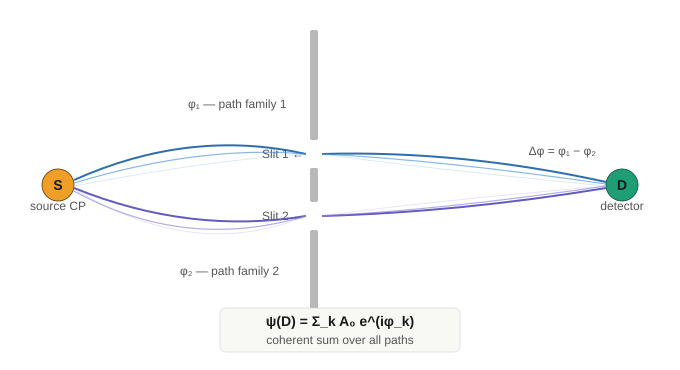
\includegraphics[width=0.90\textwidth]{qm2040b_fig1_multipath_geodesics.pdf}
\caption{Multi-path geodesics on the 600-cell lattice: double-slit
  analogy.  Source CP (amber, left) emits DI bits that simultaneously
  traverse path family~1 (blue curves, through Slit~1) and path
  family~2 (purple curves, through Slit~2) to detector (teal, right).
  Phase $\phi_1$ and $\phi_2$ accumulate along each family; the phase
  difference $\Delta\phi = \phi_1 - \phi_2$ determines the interference
  pattern at the detector.}
\label{fig:geodesics}
\end{figure}

%=====================================================================
\section{Total Amplitude and Interference}
%=====================================================================

The total amplitude at detector $d$ is the coherent sum:
\begin{equation}
\psi(d) = \sum_k A_0\,e^{i\phi_k}.
\label{eq:sum}
\end{equation}

For a double-slit geometry the dominant contributions come from two
path families (through slits 1 and~2).  The detected intensity is
\begin{equation}
I \propto |\psi_1 + \psi_2|^2
= |\psi_1|^2 + |\psi_2|^2 + 2|\psi_1||\psi_2|\cos(\Delta\phi),
\label{eq:interference}
\end{equation}
where $\Delta\phi = \phi_1 - \phi_2$.  Bright fringes occur at
$\Delta\phi = 2\pi n$; dark fringes at $\Delta\phi = \pi(2n+1)$.
This reproduces the standard double-slit result exactly.

\begin{figure}[H]
\centering
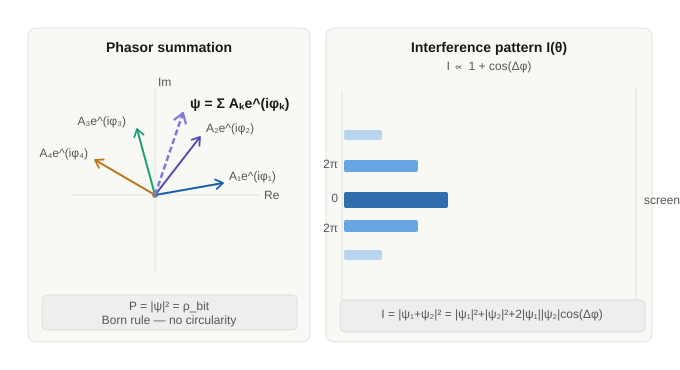
\includegraphics[width=0.90\textwidth]{qm2040b_fig2_amplitude_summation.pdf}
\caption{Coherent amplitude summation and interference pattern.
  \textit{Left:} Phasor diagram showing four path amplitudes
  $A_k e^{i\phi_k}$ (coloured arrows) summing to the resultant
  $\psi = \sum_k A_k e^{i\phi_k}$ (dashed purple arrow).
  \textit{Right:} Resulting intensity $I = |\psi|^2$ as a function of
  phase difference $\Delta\phi$, showing bright fringes at multiples
  of $2\pi$ and dark fringes at odd multiples of $\pi$.}
\label{fig:phasor}
\end{figure}

%=====================================================================
\section{Born Rule from DI-Bit Density}
%=====================================================================

\begin{theorem}[Born rule]
The probability of detection at vertex $d$ is $P(d) = |\psi(d)|^2$.
\end{theorem}

\begin{proof}
From companion~C3~\cite{abshier2026c3}, the probability of a CP state
change at a Grid Point is proportional to the local DI-bit number
density: $P \propto \rho_{\rm bit}$.  Since $\psi =
\sqrt{\rho_{\rm bit}}\,e^{i\phi}$, we have $\rho_{\rm bit} = |\psi|^2$,
and therefore $P(d) \propto |\psi(d)|^2$.
\end{proof}

\begin{remark}[No circularity]
The emission amplitude $A_0$ is defined geometrically from the source
CP state, and $\phi_k$ is the deterministic path phase~\eqref{eq:phaseedge}.
Neither is defined from a probability.  The Born rule then follows from
the identification of $|\psi|^2$ with DI-bit density --- a separate
prior result (companion~C3).
\end{remark}

%=====================================================================
\section{SSV as Which-Path Tag}
%=====================================================================

A path-dependent SSV gradient at each slit encodes which-path
information geometrically without requiring a separate quantum detector.
The additional phase shift for paths through slit~1 vs.\ slit~2 is
\begin{equation}
\Delta\phi_{\rm SSV}
= \frac{[V_{\rm SSV}({\rm S1}) - V_{\rm SSV}({\rm S2})]\,L/c}{\hbar}.
\label{eq:ssvphase}
\end{equation}
When $|\Delta\phi_{\rm SSV}|$ is large enough to distinguish the two
path families, interference is destroyed.  The SSV field itself acts
as an internal which-path marker --- a genuinely CPP-specific result.

%=====================================================================
\section{The Quantum Eraser}
%=====================================================================

Erasure restores coherence by cancelling the SSV phase difference.
Removing or symmetrising the charge distribution near one slit nulls
$\Delta\phi_{\rm SSV}$ and interference fringes reappear.

\begin{figure}[H]
\centering
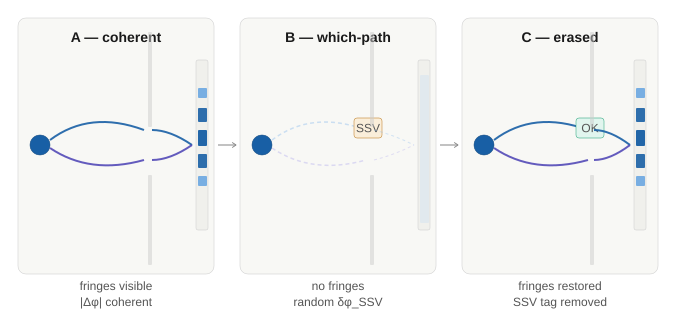
\includegraphics[width=0.90\textwidth]{qm2040b_fig3_quantum_eraser.pdf}
\caption{Quantum eraser effect.
  \textbf{A~(Coherent):} Both path families maintain coherence,
  producing bright fringes on the detector screen.
  \textbf{B~(Which-path):} An SSV gradient tag at Slit~1
  (amber label) distinguishes the paths; interference is destroyed
  and the screen shows a uniform distribution.
  \textbf{C~(Erased):} The SSV tag is removed; coherence is restored
  and fringes reappear with the same spacing and visibility as~A.}
\label{fig:eraser}
\end{figure}

%=====================================================================
\section{Connection to the Schr\"{o}dinger Equation}
%=====================================================================

The path sum~\eqref{eq:sum} is the discrete Feynman path integral.
In the continuum limit $\Delta s \to 0$ it satisfies the Schr\"{o}dinger
equation derived in Paper~2~\cite{cpp2040a}:
\begin{equation}
i\hbar\,\partial_t\psi = -\frac{\hbar^2}{2m}\nabla^2\psi + V_{\rm SSV}\psi.
\end{equation}
The local differential form (Schr\"{o}dinger) and the global integral
form (path sum) are two equivalent descriptions of the same DI-bit
hopping dynamics: the differential form arises from the stationary-phase
approximation to the path integral, and the path integral recovers
the differential form in the continuum limit.

%=====================================================================
\section{Predictions}
%=====================================================================

At all laboratory wavelengths $\lambda \gg \lP$, lattice corrections
to fringe spacing and visibility are $\mathcal{O}((\lP/\lambda)^2)
\sim 10^{-66}$ (optical) and unobservable.  At Planck-scale momenta
the dispersion relation acquires corrections of order $(p\lP/\hbar)^2$,
shifting fringe positions by $\delta\lambda/\lambda \sim (E/\EP)^2$.
These are in principle falsifiable but lie far beyond current
technology.

The CPP-specific prediction accessible in principle is the SSV
which-path effect~\eqref{eq:ssvphase}: fringe visibility should
change continuously as the charge distribution near one slit is varied,
without requiring a separate quantum detector.

%=====================================================================
\section{Conclusion}
%=====================================================================

Superposition and interference in CPP are the coherent summation of
Sea-polarization pattern contributions along all lattice paths ---
the discrete Feynman path integral.  The Born rule follows from DI-bit density
non-circularly.  The SSV encodes which-path information geometrically.
The path-sum and Schr\"{o}dinger forms are equivalent limits of the
same DI-bit hopping dynamics.  All results follow from the four CPP
postulates and the 600-cell geometry.

%=====================================================================

\section*{Acknowledgements}
The CPP programme is registered at OSF (DOI:~\url{https://doi.org/10.17605/OSF.IO/JXE8D}) and maintained at GitHub (\url{https://github.com/Hyperphysics-Institute/CPP}).

\bibliographystyle{plainnat}
\bibliography{cpp_qm_series}

\end{document}
